\documentclass[notes]{beamer}
\usetheme[numbering=fraction, progressbar=frametitle]{metropolis}
\setbeamercovered{transparent}

\usepackage[utf8]{inputenc}
\usepackage[T1]{fontenc}
\usepackage{lmodern}

\title{Zukunft der Raumfahrt}
\date{\today}
\author{Jens Juhl, Torben Mehner}
\institute{KIT}
\begin{document}
\maketitle

\begin{frame}{Inhaltsverzeichnis}
	\tableofcontents[sectionstyle=show,subsectionstyle=show]
\end{frame}

\section{Nahe Zukunft}
\subsection{NASA - Journey to Mars}
\begin{frame}{\insertsection: \insertsubsection}
	\begin{minipage}{.45\textwidth}
		Heute - Mitte 2020: \\
		\textbf{Earth Reliant} \\
		\note<1>{Earth Reliant
			\begin{itemize}
				\item ISS bis 2024
				\item Kommerzielle Raumfahrt im erdnahen Orbit
				\item Entwicklung von Systemen für interplanetare Raumfahrt
			\end{itemize}}
		
		\pause
		
		2018 - 2030: \\
		\textbf{Proving Ground} \\
		\note<2>{
			Proving Ground
			\begin{itemize}
				\item Regelmäßige, bemannte Missionen im Mondorbit
				\item Durch jahrelange Missionen beweisen, dass Habitate im 
				weiten All funktionieren
				\item Einfangen eines Asteroids und Platzierung im Mond-Orbit. 
				Dann sollen Astronuten robotergestützt Proben nehmen.
			\end{itemize}
			}
		\pause
		
		Heute - 2030 und länger: \\
		\textbf{Earth Independant}
		\note<3>{
			Earth Independant
			\begin{itemize}
				\item Missionen erforschen Mars
				\item Demonstration von Eintritt, Landung und 
				In-Situ-Ressourcenverwendung
				\item Unbemannte Missionen mit Rückkehr zum Mars
				\item In den frühen 2030ern: Menschen sollen den Mars umrunden
			\end{itemize}
		}
		
	\end{minipage} \quad
	\begin{minipage}{.5\textwidth}
		\only<1>{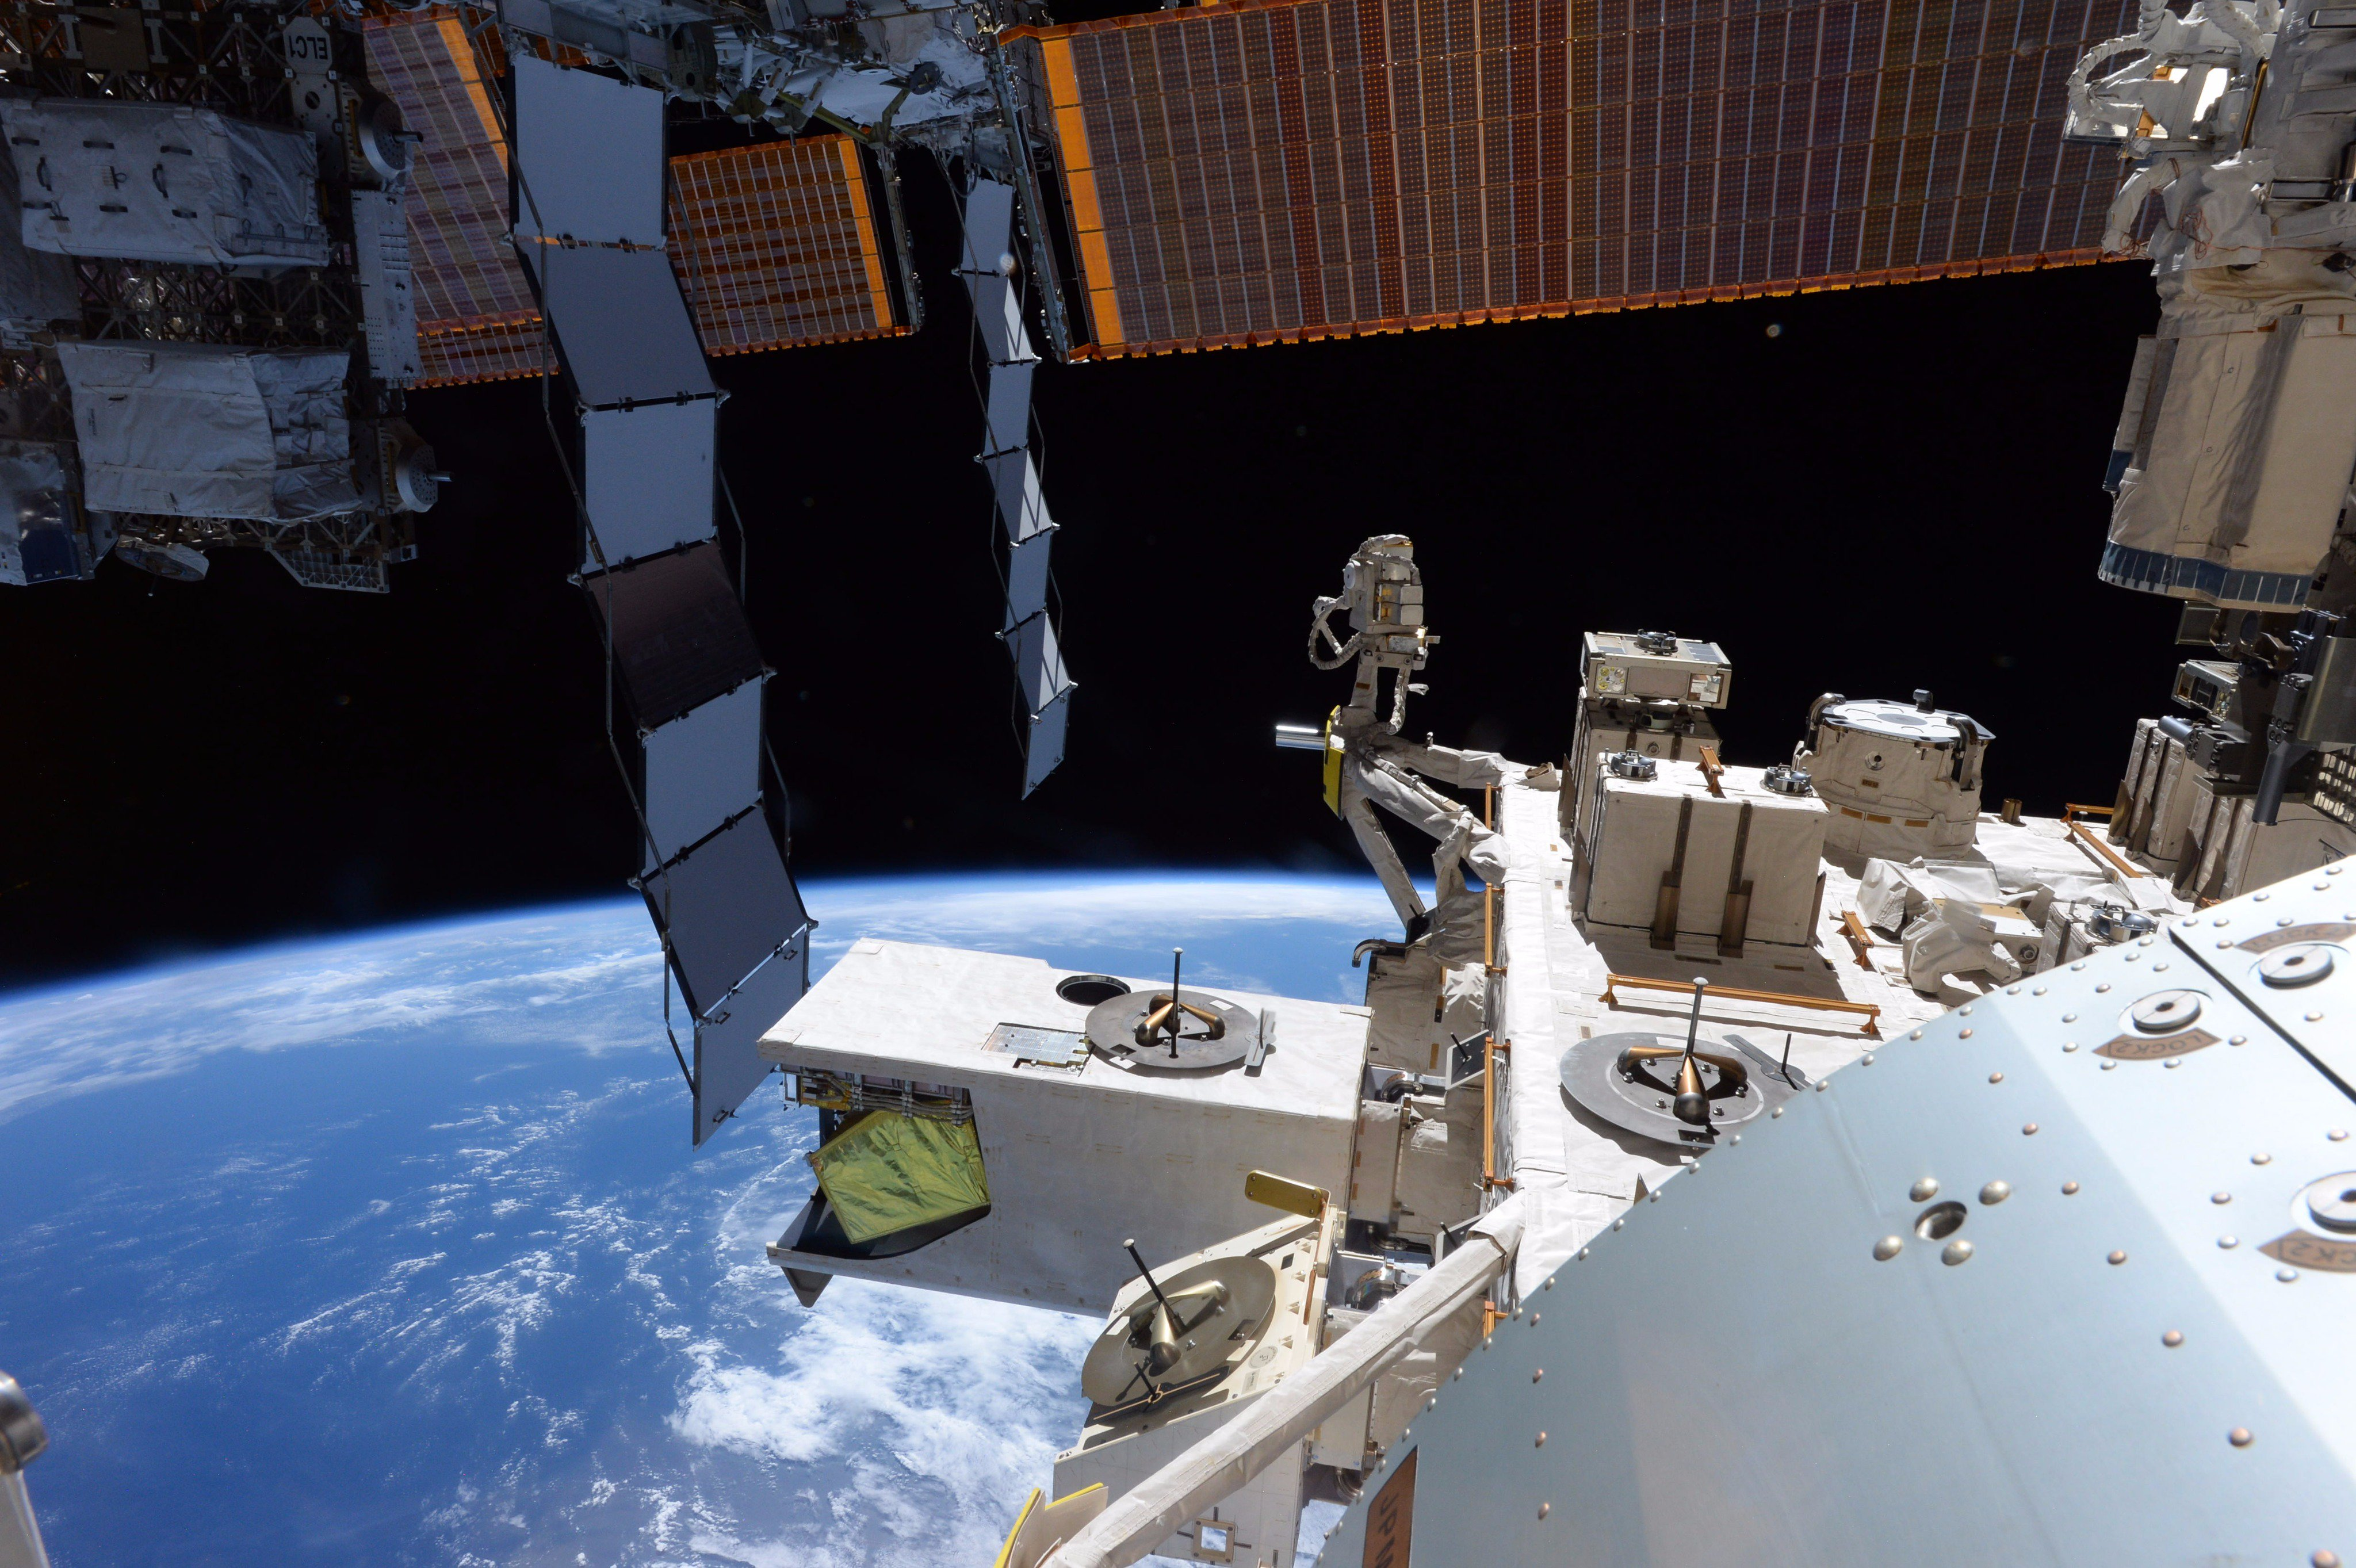
\includegraphics[width=\linewidth]{iss}
		
		{\tiny An Astronaut's View From the 'Corner Office',
		\\ Quelle: nasa.gov}}
		\only<2>{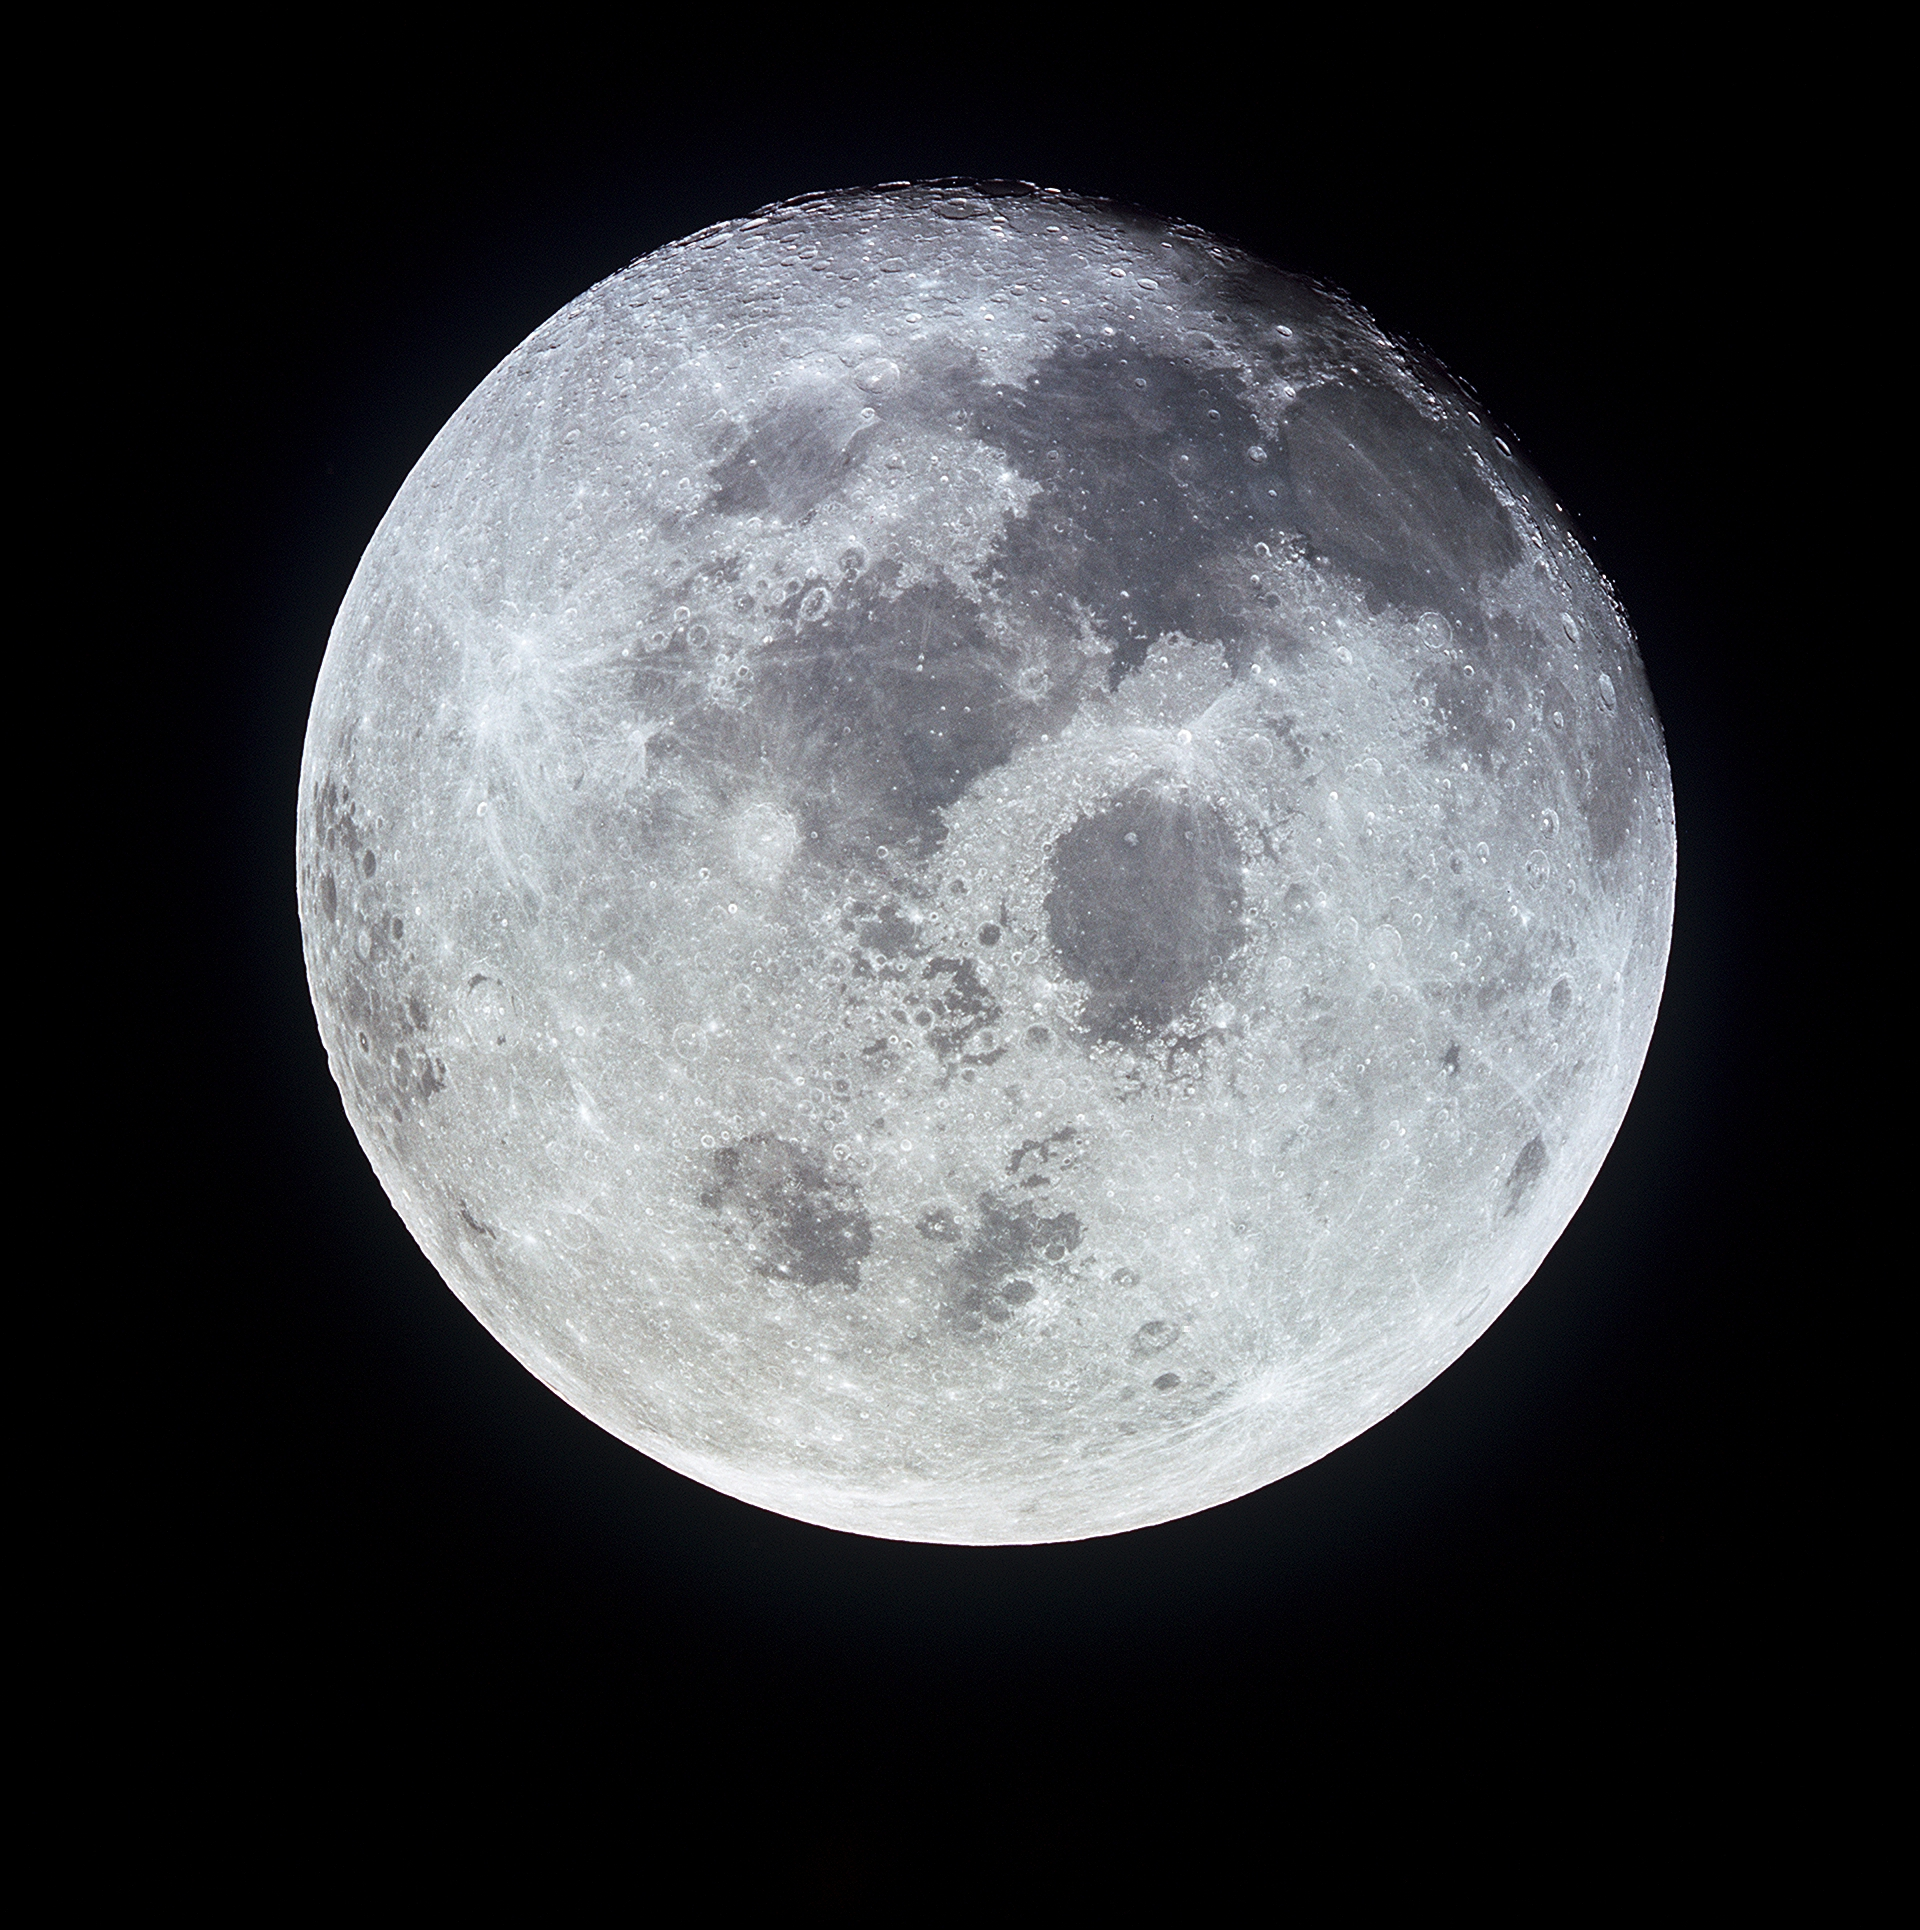
\includegraphics[width=\linewidth]{moon}
			
		{\tiny Photo of full Moon taken at Apollo 11 mission,
		\\ Quelle: nasa.gov}}

		\only<3>{\includegraphics[width=\linewidth]{mars}
			
		{\tiny Curiosity Self-Portrait at 'Murray Buttes',
		\\ Quelle: nasa.gov}}
	\end{minipage}
\end{frame}

\subsection{ESA und Roscosmos - ExoMars}
\begin{frame}{\insertsection: \insertsubsection}
	\begin{minipage}{.45\textwidth}
		
		Heute - 2024: \\
		\textbf{ISS} \\
		
		\pause
		
		2016 - 2022: \\
		\textbf{TGO und Schiaparelli} \\
		\note<2>{Schiaparelli
			\begin{itemize}
				\item TGO: Trace Gas Orbiter
				\item Nachweis von Stoffwechselprodukten
				\item Schiaparelli bei Landung (Oktober 2016) zerschellt
			\end{itemize}}
		
		\pause
		
		Ab 2020: \\
		\textbf{ExoMars Rover} \\
		\note<3>{ExoMars Rover
			\begin{itemize}
				\item Sucht Leben auf dem Mars
				\item Hat einen Bohrer um tiefe Schichten zu erreichen (2m 
				Maximum)
				\item Hat viele Analyseinstrumente um Zusammensetzung des 
				Bodens zu bestimmen
				\item Fährt autonom bis zu 100m pro Sol (Mars-Tag). Verbindung 
				zur ESA nur ein bis zwei mal pro Sol möglich.
			\end{itemize}}
				
		\end{minipage} \quad
		\begin{minipage}{.5\textwidth}
			\only<1>{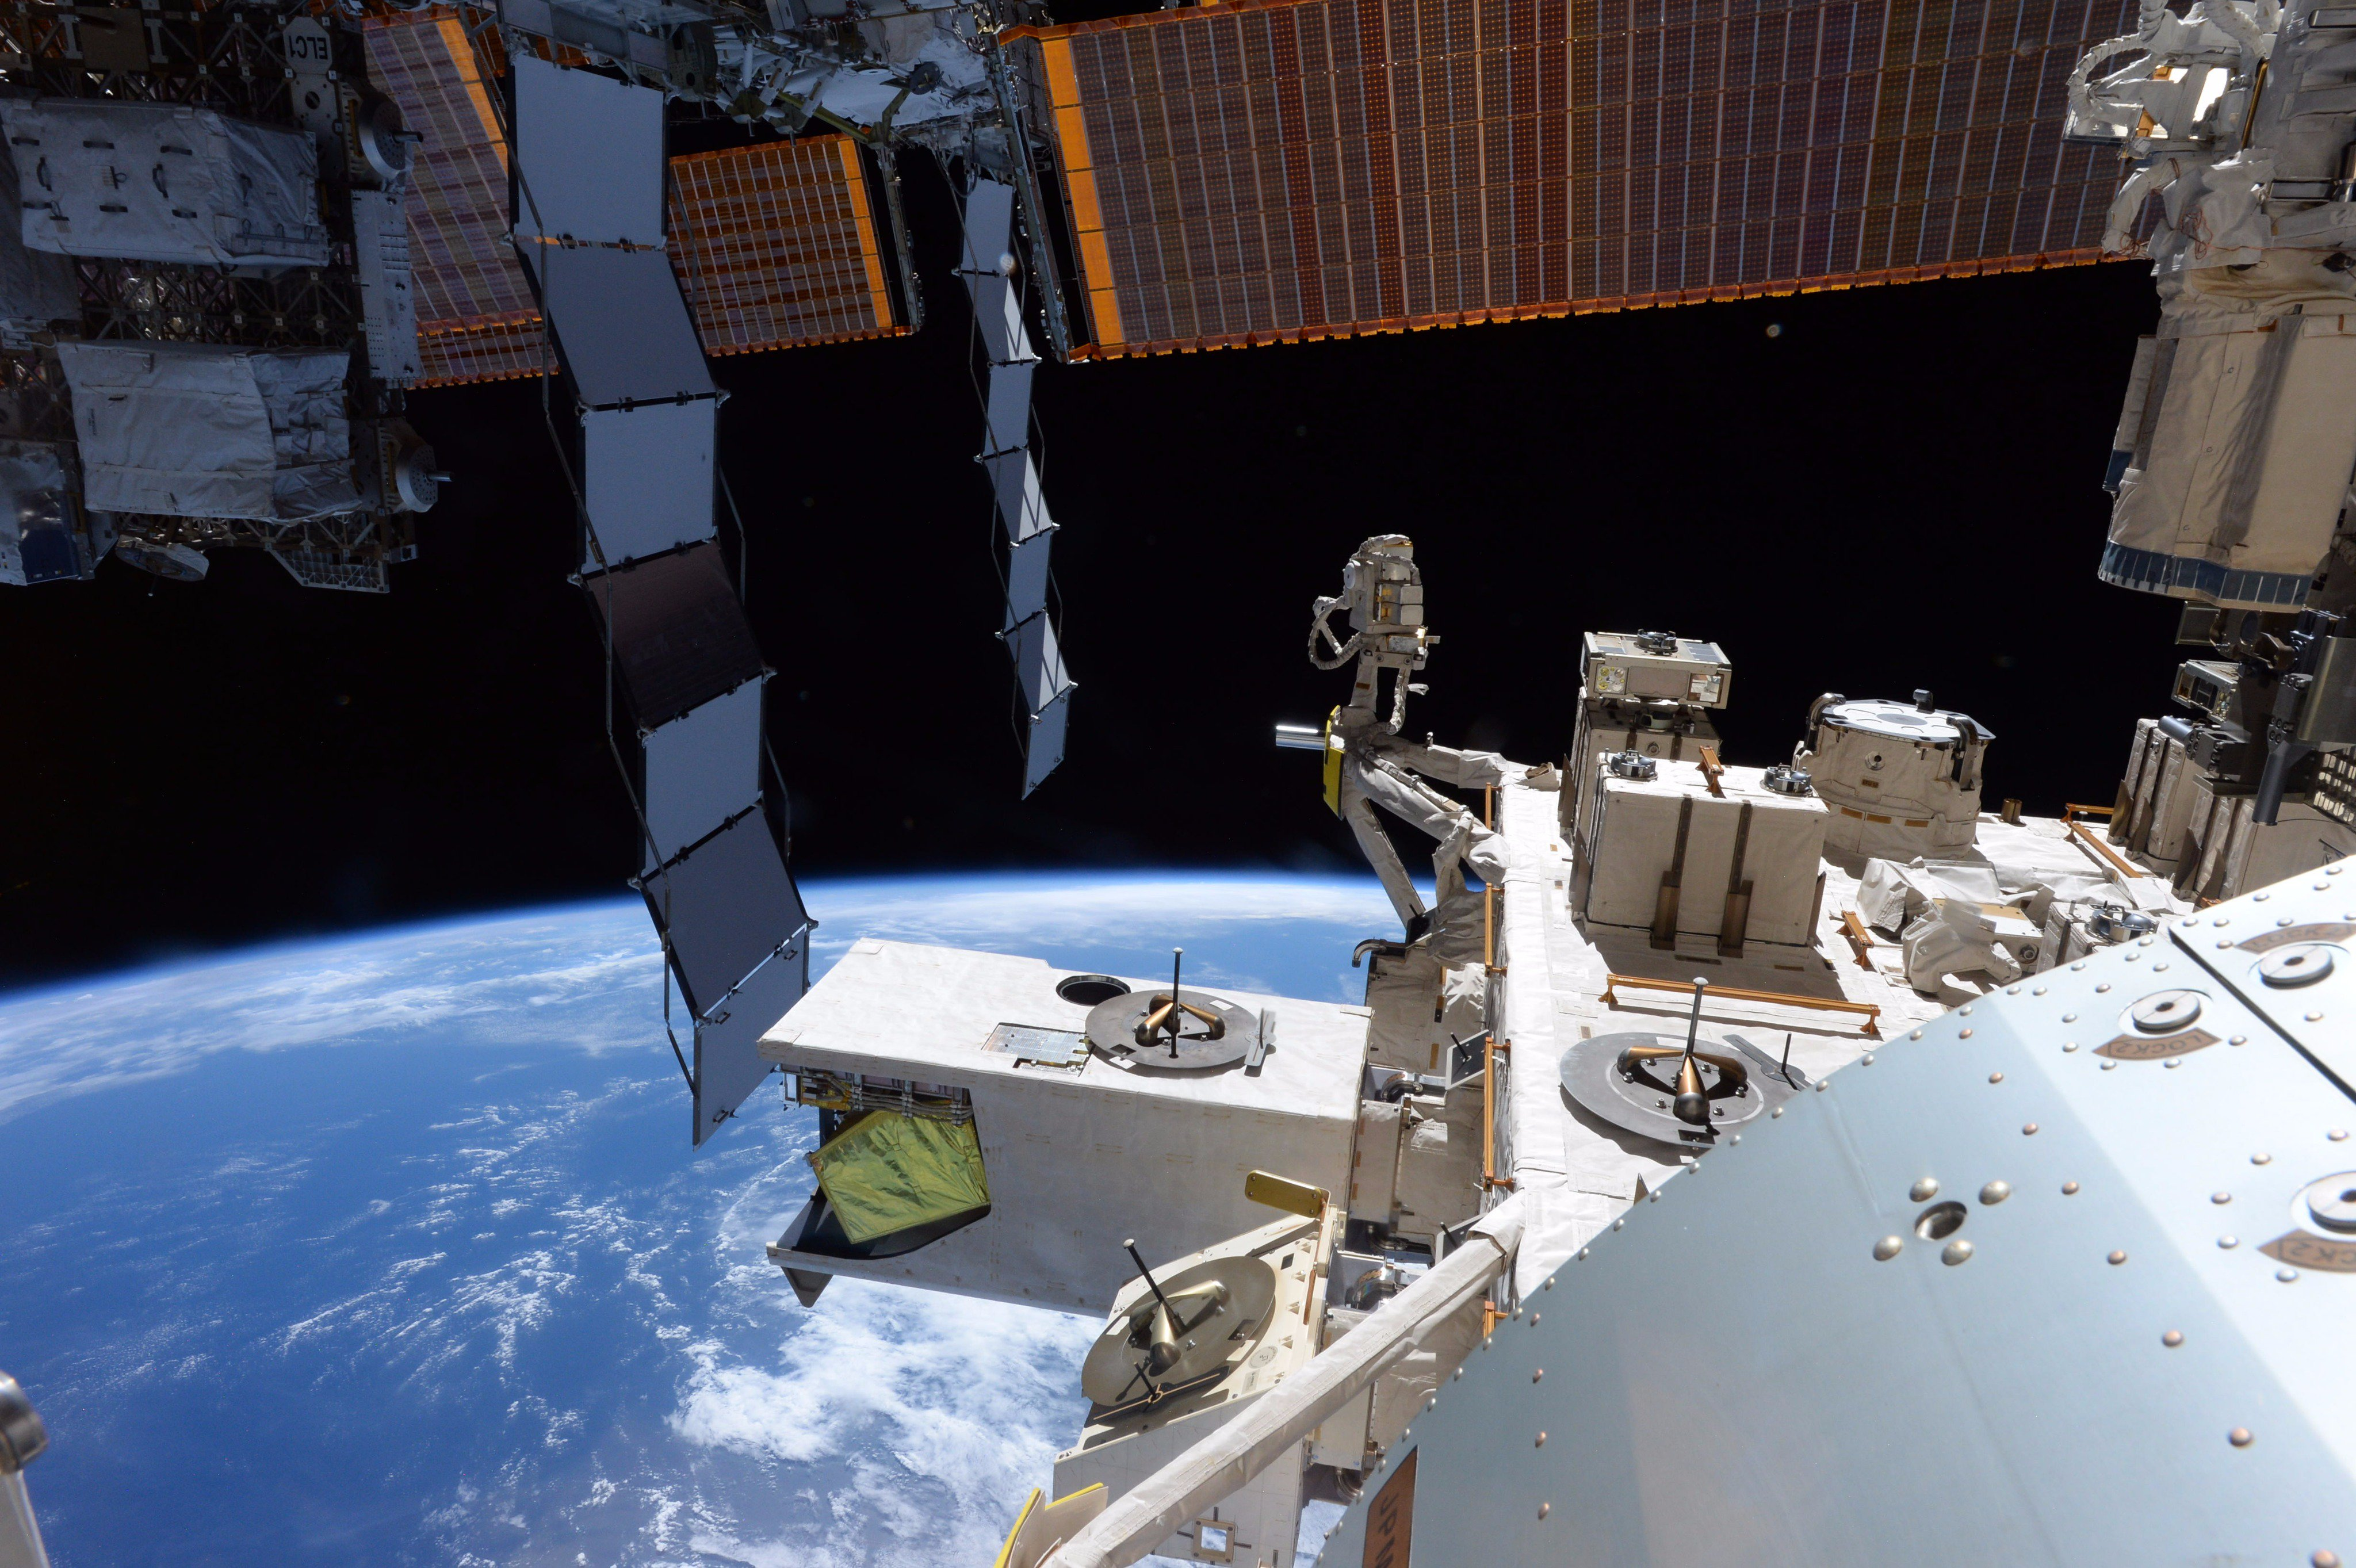
\includegraphics[width=\linewidth]{iss}
				
				{\tiny An Astronaut's View From the 'Corner Office',
					\\ Quelle: nasa.gov}}
			\only<2>{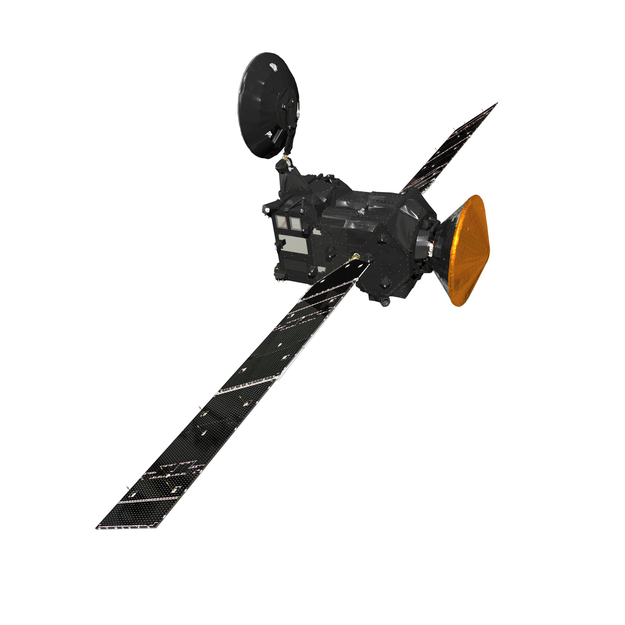
\includegraphics[width=\linewidth]{schiaparelli}
				
				{\tiny ExoMars 2016: Trace Gas Orbiter and Schiaparelli,
					\\ Quelle: esa.int}}
			\only<3>{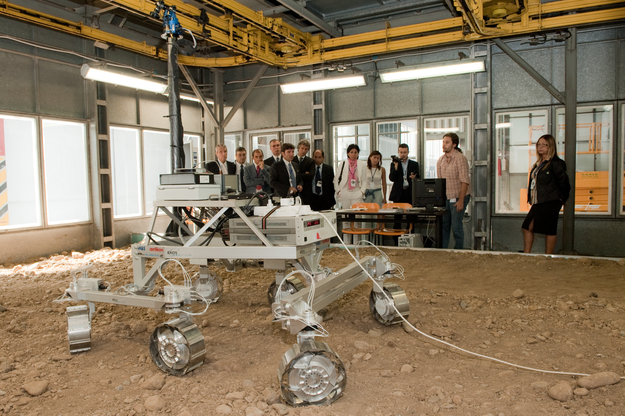
\includegraphics[width=\linewidth]{exomars}
				
				{\tiny The ExoMars Rover Prototype,
					\\ Quelle: esa.int}}
		\end{minipage}
	\end{frame}
	
\subsection{ESA - Kommerziell}
\begin{frame}{\insertsection: \insertsubsection}
	\begin{minipage}{.45\textwidth}
		
		Heute - 2020: \\
		\textbf{Umrüsung auf Ariane VI} \\
		
		\note{
			\begin{itemize}
				\item Preis pro kg bei 11to: 8000 Euro (4 Booster)
				\item Preis pro kg bei 4,5to: 16700 Euro (2Booster)
			\end{itemize}
			}
				
			\end{minipage} \quad
			\begin{minipage}{.5\textwidth}
				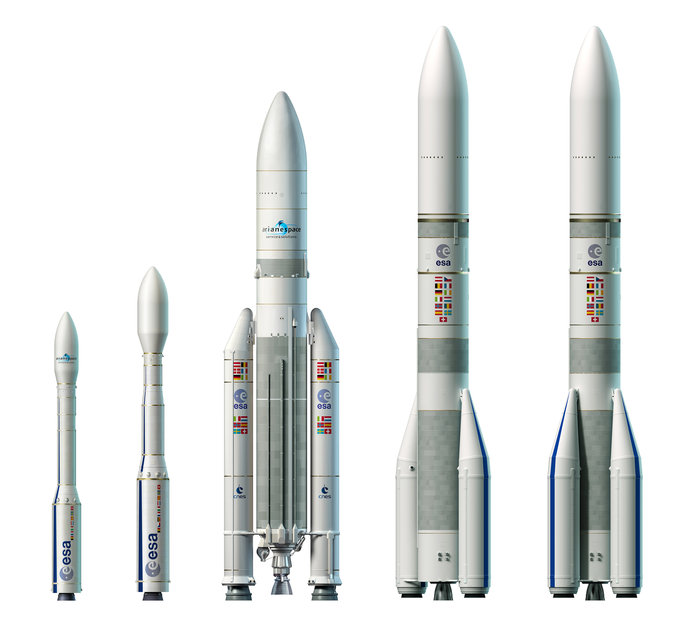
\includegraphics[width=\linewidth]{arianevi}
					
					{\tiny Artist's view of Vega, Vega-C, Ariane 5 ECA and the 
					two configurations of Ariane 6,
						\\ Quelle: esa.int}
			\end{minipage}
\end{frame}

\subsection{SpaceX}
\begin{frame}{\insertsection: \insertsubsection}
	\begin{minipage}{.45\textwidth}
		
		Seit Heute: \\
		\textbf{Falcon 9 und Falcon Heavy} \\
		
		\note<1>{
			\begin{itemize}
				\item Falcon 9 pro kg bei 8,5to: 7500 Euro
				\item Falcon Heavy pro kg bei 26,7to: 3400 Euro
			\end{itemize}
		}
		
		\pause
		
		Ab 2022: \\
		\textbf{Making Life Multiplanetary} \\
		
		\note<2>{
			\begin{itemize}
				\item 2022: unbemannte Versorgungsmission
				\item 2024: erste bemannte Mission
			\end{itemize}
		}
		
		\pause
		
		Ab 2022: \\
		\textbf{BFR | Earth to Earth} \\
		
		\note<3>{
			\begin{itemize}
				\item BFR: Rakete der Marsmission
				\item Slogan: Um die halbe Welt in weniger als 30 Minuten
			\end{itemize}
		}
		
		
	\end{minipage} \quad
	\begin{minipage}{.5\textwidth}
		\only<1>{\begin{center}
			
\includegraphics[height=.93\linewidth]{falcon9} \hspace{24pt}
			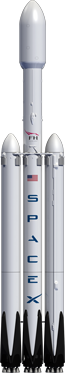
\includegraphics[height=\linewidth]{falconheavy}
		\end{center}		
		
		{\tiny Falcon 9 und Falcon Heavy,
			\\ Quelle: spacex.com}}
	
		\only<2>{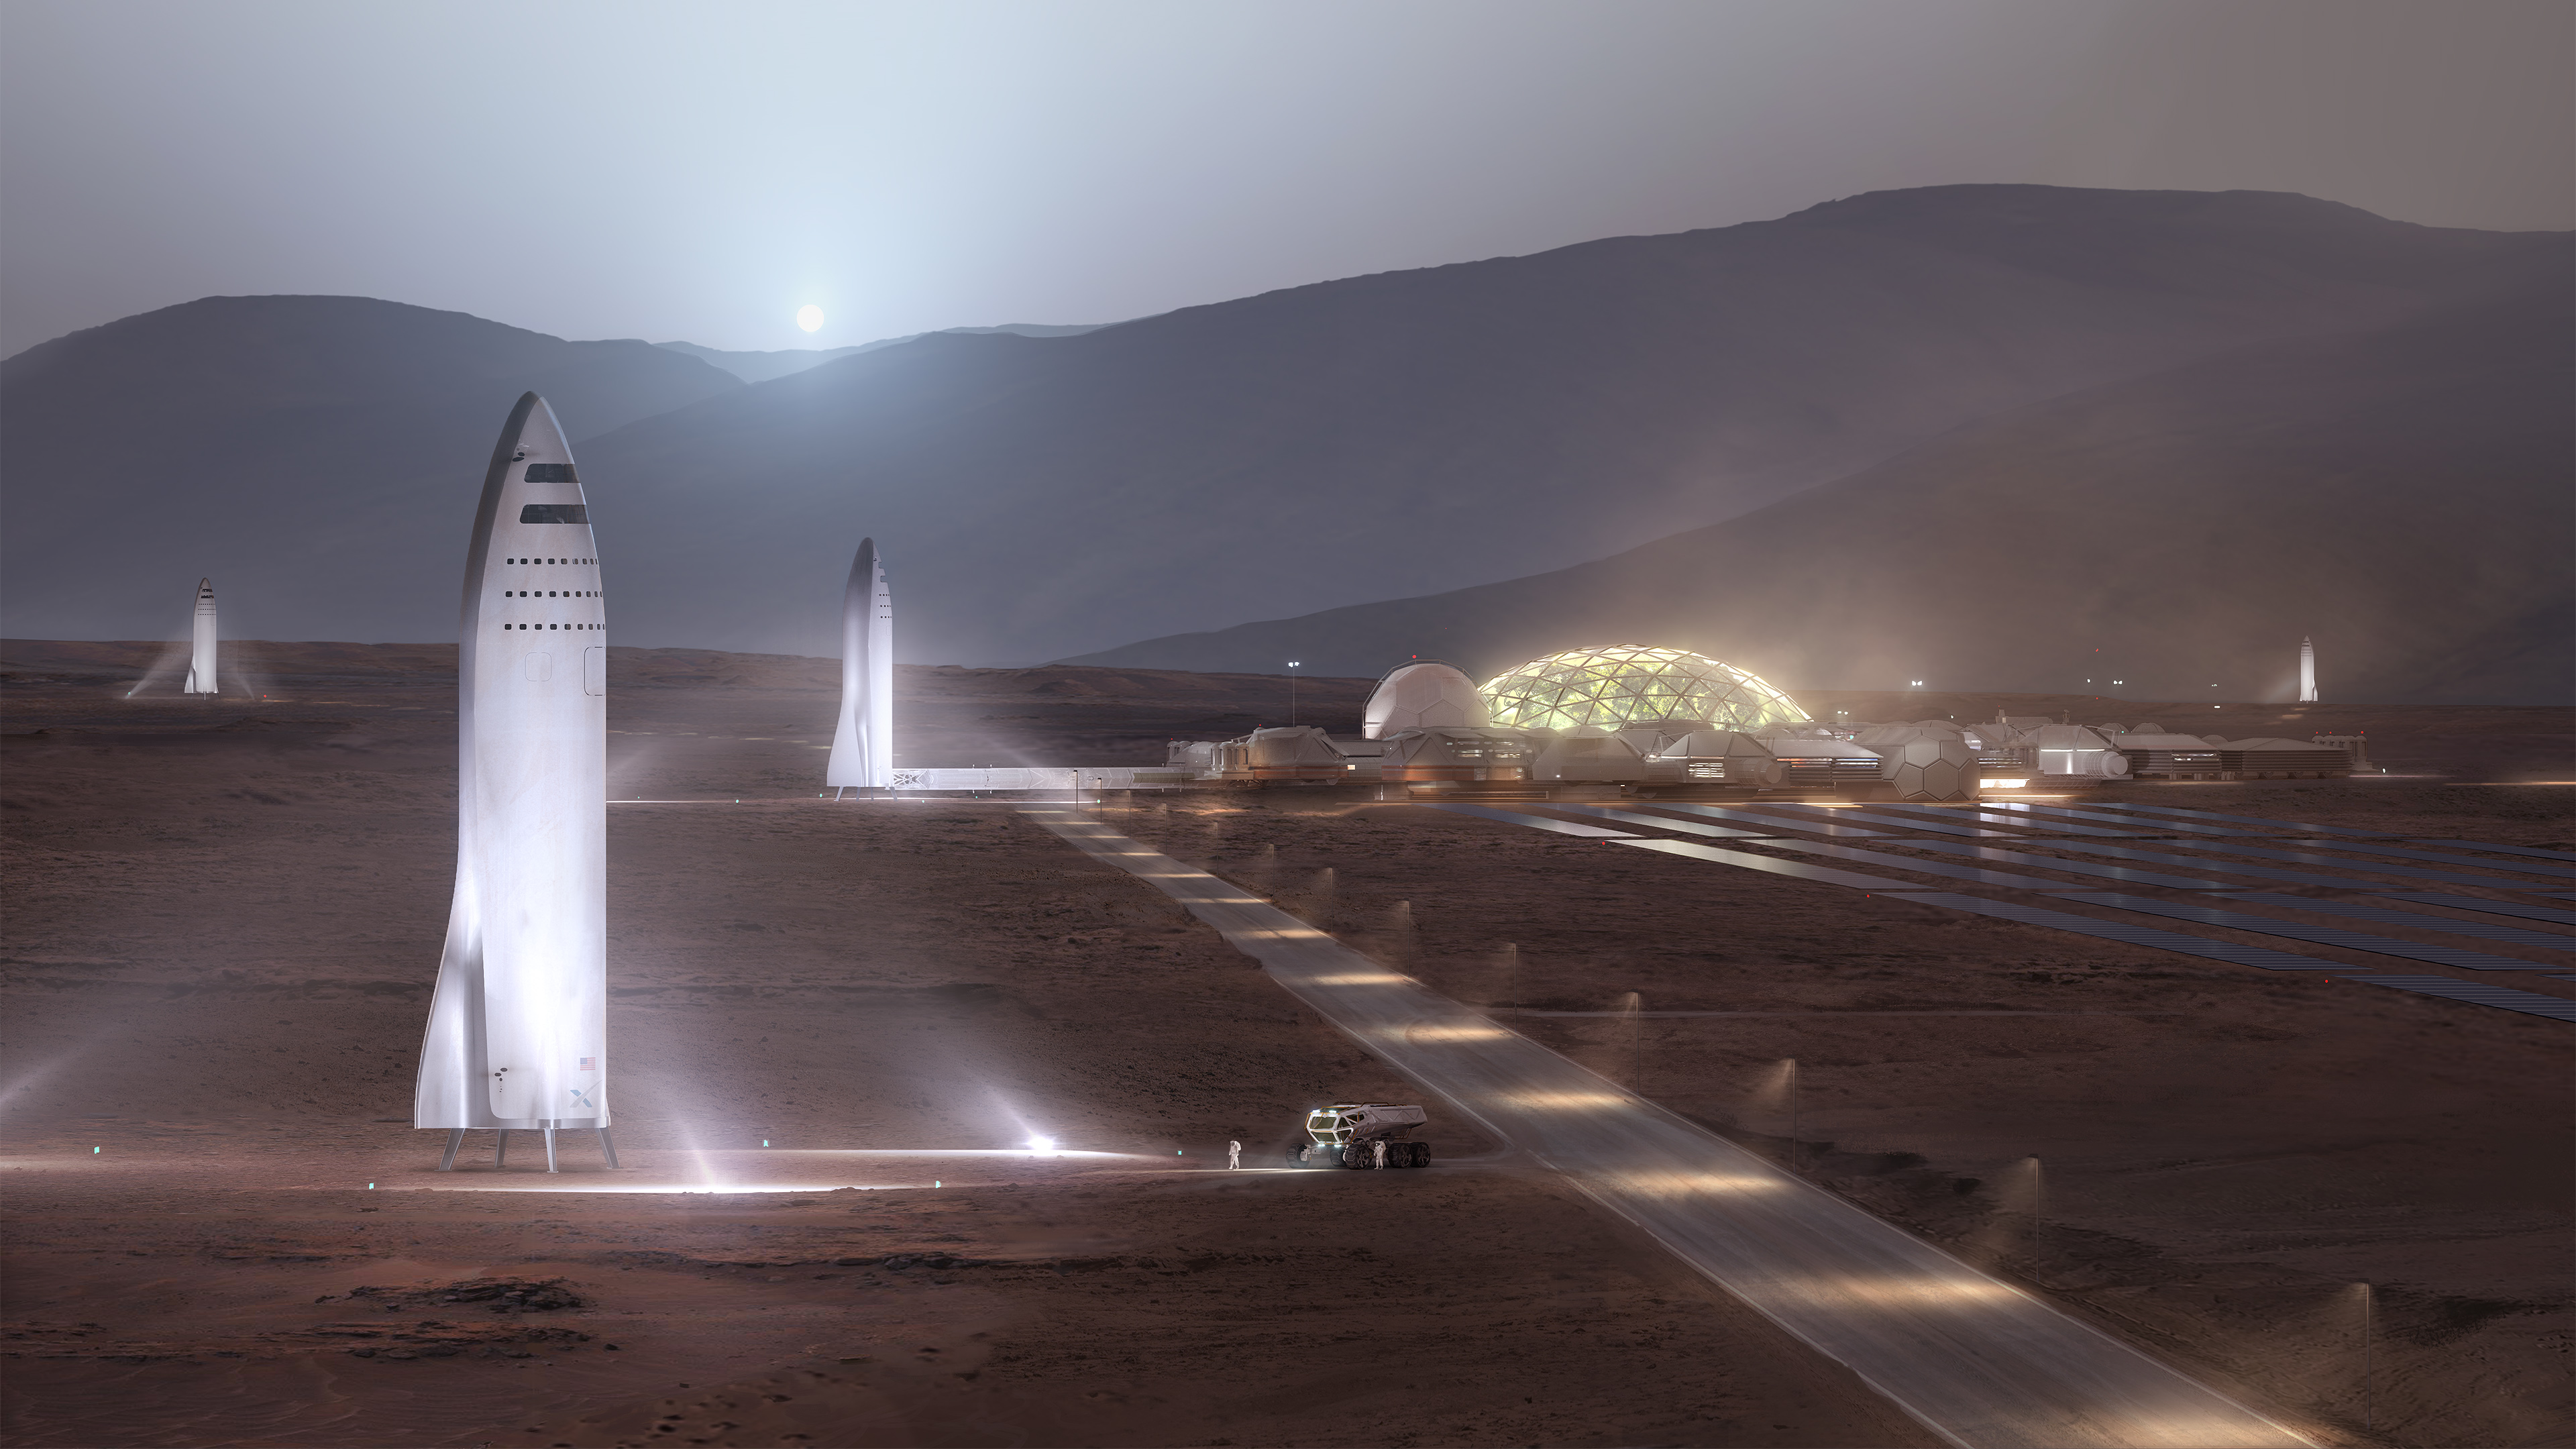
\includegraphics[width=\linewidth]{spacexmars}
			
			{\tiny Missions to Mars,
				\\ Quelle: spacex.com}}
		
		\only<3>{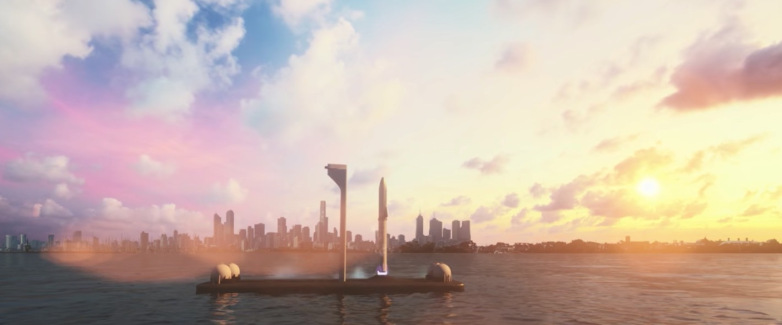
\includegraphics[width=\linewidth]{earthtoearth}
			
			{\tiny BFR: Earth to Earth,
				\\ Quelle: spacex.com}}
	\end{minipage}
\end{frame}

\subsection{CNSA}
\begin{frame}{\insertsection: \insertsubsection}
	Goodbye, world!
\end{frame}

\section{Ferne Zukunft}
\subsection{Erster Unterpunkt}
\begin{frame}{\insertsection: \insertsubsection}
	Goodbye, world!
\end{frame}

\end{document}